\section{Pré-traitements : localisation et extraction des chiffres manuscrits}

Dans l'exemple étudié, la façon la plus simple de localiser les chiffres consiste d'abord à rechercher, à partir de l'histogramme de projections horizontales de pixels noirs, les plages correspondant à un nombre de pixels noirs non nul. Le début et la fin de chaque plage détectée sur l'histogramme des projections horizontales définissent une ligne de chiffres dans l'image. En appliquant le même principe (mais à partir d'un histogramme de projections verticales) sur chaque ligne détectée, on peut alors déterminer l'emplacement de chaque chiffre de l'image.

\subsection{Recherche des lignes}
Le principe est très simple, puisqu'il suffit dans un premier temps de parcourir chaque ligne pour vérifier qu'elle contient un pixel noir ou non. Pour accélérer le processus et parcourir rapidement l'image, un histogramme du nombre de pixels noirs est récupéré. Ceci est possible facilement car l'image est déjà binaire. On peut alors remarquer de façon évidente les différentes lignes. Les valeurs de celles-ci (début et fin) sont alors sauvegardées pour être réutilisées lors de la recherche des colonnes.

\begin{figure}[hm]
	\begin{center}
		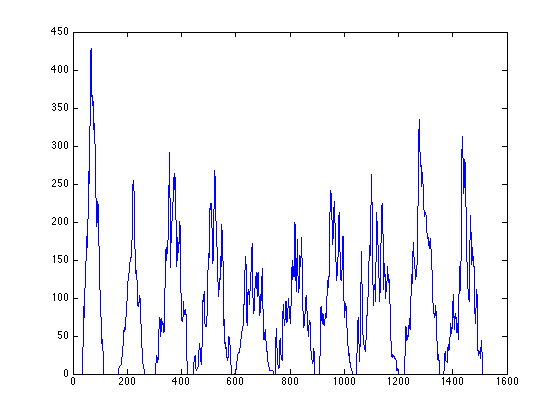
\includegraphics[width=0.8\textwidth]{img/10-black-level.png} 
	\end{center}
	\caption{Histogramme du niveau de noir}
\end{figure}
\newpage
\subsection{Recherche des colonnes pour chaque ligne}
Le même principe utilisé précédemment est recommencé, avec cette fois un histogramme du niveau de noir sur chaque colonne, pour une ligne unique (soit une ligne de chiffre). On obtient alors plusieurs histogrammes semblables au précédent, qui permettent d'obtenir un tableau avec les colonnes englobant chaque chiffre pour chaque ligne. 

\subsection{Détermination du rectangle englobant}
On pourrait penser qu'il n'y a plus d'étapes de découpe et qu'il faut uniquement assembler les coordonnées colonnes avec celles des lignes, mais il est nécessaire de repasser pour chaque chiffre dans le découpage des lignes, car ils possèdent un profil vertical beaucoup trop grand pour certains (puisqu'il s'agit du plus haut et plus bas chiffre pour chaque ligne). Ainsi, en effectuant une découpe plus précise, on obtient au final le résultat suivant.

\begin{figure}[hm]
	\begin{center}
		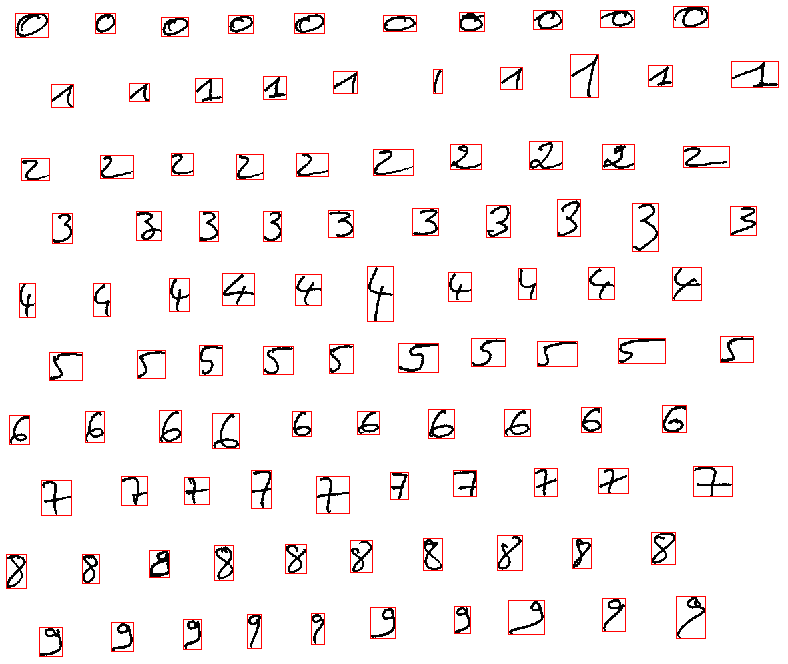
\includegraphics[width=0.8\textwidth]{img/11-final-cut.png} 
	\end{center}
	\caption{Résultat des découpes}
\end{figure}

\subsection{Avantages et inconvénients d'une telle méthode}
Cette méthode de localisation par projection est avantageuse puisque dans le cas ci présent, elle fournit un résultat parfait quant à la découpe des chiffres. Seulement, celle-ci peut perdre énormément en pertinence si les lignes de chiffres  n'étaient pas aussi droites.\\
Imaginons deux lignes consécutives, écrites de façon à ce qu'elles montent toutes les deux vers le haut. On se retrouve avec le premier chiffre de la première ligne qui se retrouve à la même hauteur que le dernier chiffre de la deuxième ligne. Ainsi, la méthode de l'histogramme ne convient pas du tout car on ne pourrait faire la différence entre les deux lignes.\\
On peut également remarquer que cette méthode devient vite lourde pour les images de grande taille et comprenant un nombre important de caractères (en plus de chiffres), et il serait donc pertinent de trouver une méthode plus optimisée.